\begin{figure}[H]
    \centering

    \tikzset{
    max node/.style={circle,draw,inner sep=5},
    min node/.style={circle,draw,inner sep=5, fill=gray},
    bold/.style={line width=1mm},
    thin/.style={line width=0.2mm}
    }

    % Specify spacing for each level of the tree
    \tikzstyle{level 1}=[level distance=1.7mm,sibling distance=4mm]
    \tikzstyle{level 2}=[level distance=1.7mm,sibling distance=2mm]
    
    \begin{tabular}{cc}
        
    \begin{subfigure}[b]{0.4\textwidth}
        \centering
        \resizebox{\textwidth}{!}{
            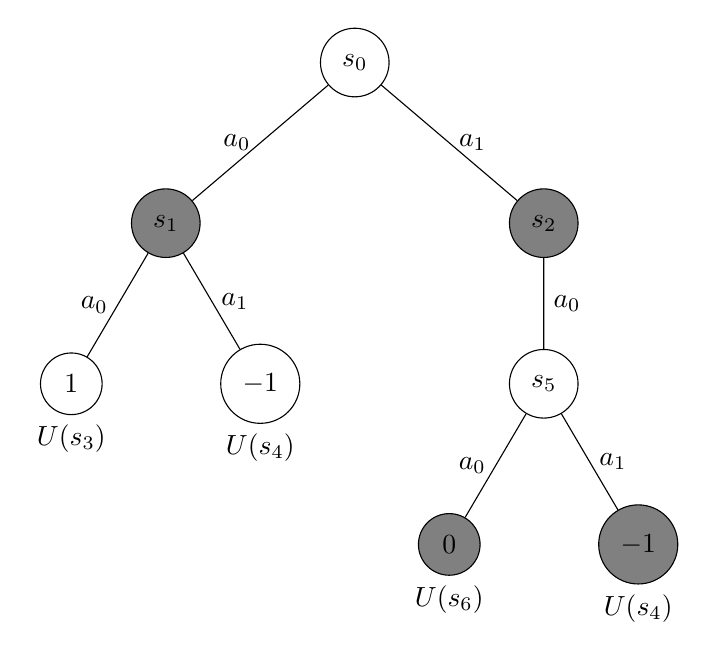
\begin{tikzpicture}[scale=12]
                \node(0)[max node]{$s_0$}
                child{node(1)[min node]{$s_1$}
                    child{node[max node, label=below:{$U(s_3)$}]{$1$}
                        edge from parent node[left]{$a_0$}
                    }
                    child{node[max node, label=below:{$U(s_4)$}]{$-1$}
                        edge from parent node[right]{$a_1$}
                    }
                    edge from parent node[left]{$a_0$}
                }
                child{node(2)[min node]{$s_2$}
                    child{node[max node]{$s_5$}
                        child{node[min node, label=below:{$U(s_6)$}]{$0$}
                            edge from parent node[left]{$a_0$}
                        }
                        child{node[min node, label=below:{$U(s_4)$}]{$-1$}
                            edge from parent node[right]{$a_1$}
                        } 
                        edge from parent node[right]{$a_0$}
                    }
                    edge from parent node[right]{$a_1$}
                };
            \end{tikzpicture}
        }
    \end{subfigure}
    &
    \begin{subfigure}[b]{0.4\textwidth}
        \centering
        \resizebox{\textwidth}{!}{
            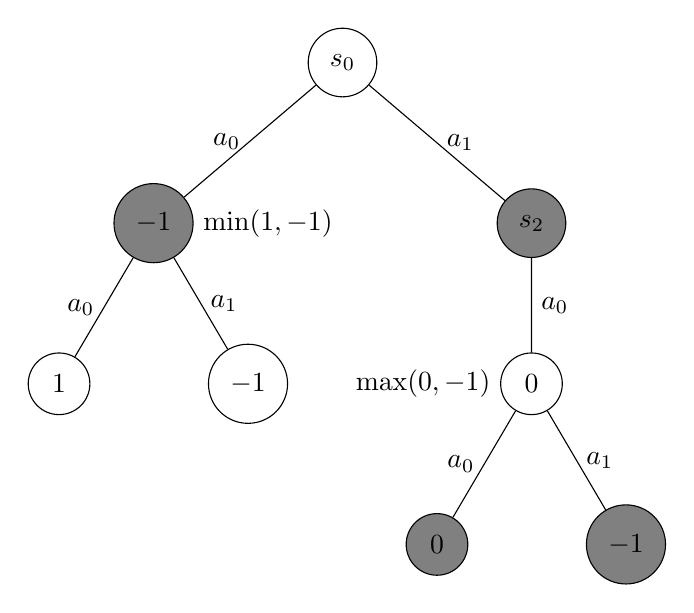
\begin{tikzpicture}[scale=12]
                \node(0)[max node]{$s_0$}
                child{node(1)[min node, label=right:{$\min(1, -1)$}]{$-1$}
                    child{node[max node]{$1$}
                        edge from parent node[left]{$a_0$}
                    }
                    child{node[max node]{$-1$}
                        edge from parent node[right]{$a_1$}
                    }
                    edge from parent node[left]{$a_0$}
                }
                child{node(2)[min node]{$s_2$}
                    child{node[max node, label=left:{$\max(0, -1)$}]{$0$}
                        child{node[min node]{$0$}
                            edge from parent node[left]{$a_0$}
                        }
                        child{node[min node]{$-1$}
                            edge from parent node[right]{$a_1$}
                        } 
                        edge from parent node[right]{$a_0$}
                    }
                    edge from parent node[right]{$a_1$}
                };
            \end{tikzpicture}
        }
    \end{subfigure}
    \\
    \begin{subfigure}[b]{0.4\textwidth}
        \centering
        \resizebox{\textwidth}{!}{
            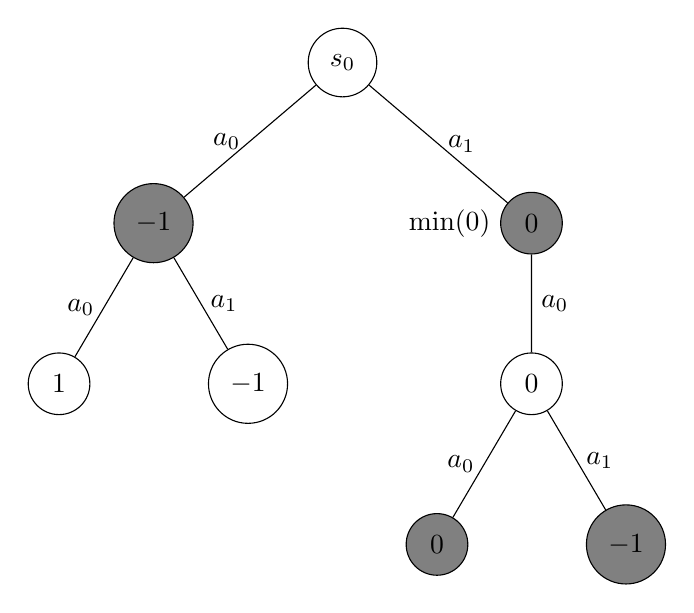
\begin{tikzpicture}[scale=12]
                \node(0)[max node]{$s_0$}
                child{node(1)[min node]{$-1$}
                    child{node[max node]{$1$}
                        edge from parent node[left]{$a_0$}
                    }
                    child{node[max node]{$-1$}
                        edge from parent node[right]{$a_1$}
                    }
                    edge from parent node[left]{$a_0$}
                }
                child{node(2)[min node, label=left:{$\min(0)$}]{$0$}
                    child{node[max node]{$0$}
                        child{node[min node]{$0$}
                            edge from parent node[left]{$a_0$}
                        }
                        child{node[min node]{$-1$}
                            edge from parent node[right]{$a_1$}
                        } 
                        edge from parent node[right]{$a_0$}
                    }
                    edge from parent node[right]{$a_1$}
                };
            \end{tikzpicture}
        }
    \end{subfigure}
    &
    \begin{subfigure}[b]{0.4\textwidth}
        \centering
        \resizebox{\textwidth}{!}{
            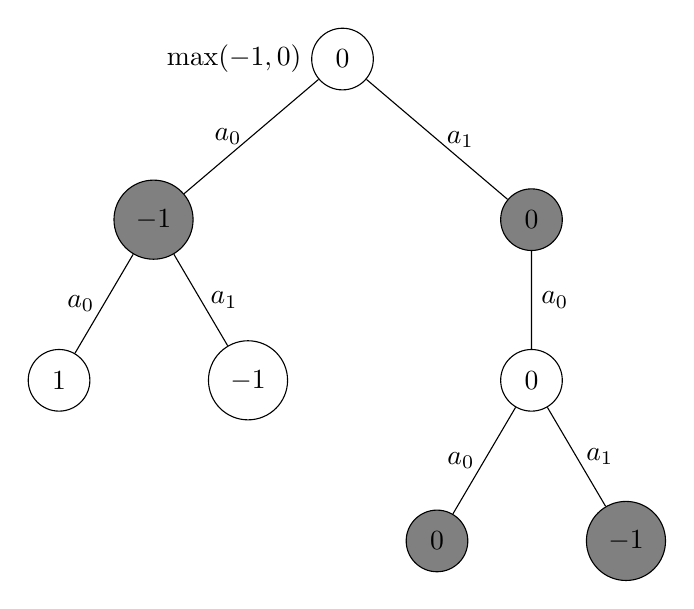
\begin{tikzpicture}[scale=12]
                \node(0)[max node, label=left:{$\max(-1, 0)$}]{$0$}
                child{node(1)[min node]{$-1$}
                    child{node[max node]{$1$}
                        edge from parent node[left]{$a_0$}
                    }
                    child{node[max node]{$-1$}
                        edge from parent node[right]{$a_1$}
                    }
                    edge from parent node[left]{$a_0$}
                }
                child{node(2)[min node]{$0$}
                    child{node[max node]{$0$}
                        child{node[min node]{$0$}
                            edge from parent node[left]{$a_0$}
                        }
                        child{node[min node]{$-1$}
                            edge from parent node[right]{$a_1$}
                        } 
                        edge from parent node[right]{$a_0$}
                    }
                    edge from parent node[right]{$a_1$}
                };
            \end{tikzpicture}
        }
    \end{subfigure}

    \end{tabular}
    \caption{Backpropagation of MiniMax values. Notice that when the
    backpropagation is finished, there is a path from the root to 
    a leaf containing identical values. This is known as the principal
    variation, and is the path that the agents will take if both are 
    playing optimally.}
    \label{fig:minimax_example}

\end{figure}
